\documentclass[french,a4paper]{report}
 
% - taille de la fonte    : 10pt, 11pt, 12pt
% - recto ou recto-verso    : oneside, twoside
 
% Chargement d'extensions
\usepackage[utf8]{inputenc}    
\usepackage{graphicx}
\usepackage{amsmath}
\usepackage{amsfonts}
\usepackage{epsfig}
\usepackage{color}
\usepackage{natbib}
\usepackage{mathrsfs} 
% \usepackage[french]{babel}    
 
% Informations le titre, le(s) auteur(s), la date
\title{X-Light - Software for stress analysis with X-ray diffraction techniques}
\author{User guide}
\date{\today}

 
 
 
\begin{document}

\sloppy
 
% \maketitle

\begin{titlepage}
\centering
\vfill
{\Huge
X-Light\\
Software for stress analysis\\
\Large
\vskip1cm
User guide\\
\vskip1cm
\today\\
}    
\vfill
\scalebox{0.2}{
\includegraphics{figures/X-Light.png}}
\vfill
\vfill
\end{titlepage}

\tableofcontents 


\chapter{Introduction}

X-Light is an open source software dedicated to the evaluation of stresses from X-ray diffraction data. The software, which is developed in Python, offers different functions that can be called from a Graphical User Interface (GUI). X-Light allows importing X-ray diffraction data collected with point, line and area detectors. Once X-ray diffraction data has been imported, an optimization procedure allows determining peak positions. Finally, these positions can be used as an input to evaluate the stress state and the corresponding uncertainties.

This document is a guide for users of the X-Light software. The method used for stress calculation is detailed in the first part of this guide. The operation of X-Light is then presented. 
    

\chapter{Stress analysis with X-ray diffraction techniques}

This first chapter aims at briefly presenting the method of stress analysis used within X-Light as well as specifying the conventions used \footnote{This chapter is not intended to be a detailed course document on the subject of stress analysis with X-ray diffraction techniques. The interested reader is referred to the reference literature dedicated to this subject.}. This mainly involves providing the X-Light user with essential information on the method used so that he/she can correctly interpret the results obtained. 


\section{Geometry conventions}

Stress analysis with X-ray diffraction relies on the acquisition of the signal diffracted by a sample when illuminated by a monochromatic light source. The acquisition of the diffracted signal requires the use of a detector (point, linear or surface), which measures the intensity of the light beam diffracted by the sample. Each point of the detector is associated with a measurement direction (that of the diffraction vector), represented by a unit vector $\boldsymbol n$. For area detectors, a point of the detector corresponds to two angles called $2 \theta$ and $\gamma$. The values of these angles depend both on the pixel considered and on the angular position $\alpha$ of the detector on the goniometric circle (see Figure \ref{fig_bases}). For the specific cases of point or linear detectors, the angle $\gamma$ is zero while the angle $2 \theta$ is equal to the angle $\alpha$. 

The components of the measurement direction are easily determined within the base $\mathcal{E}$ attached to the diffraction goniometer from the angles $\theta$ and $\gamma$. As shown in Figure \ref{fig_bases}, the base $\mathcal{E}$ is constructed from three mutually orthogonal unit vectors $(\boldsymbol e_1$, $\boldsymbol e_2$ and $\boldsymbol e_3)$. Specifically, the vector $\boldsymbol e_2$ is parallel to the incident beam, the vector $\boldsymbol e_1$ is orthogonal to the goniometric circle while the vector $\boldsymbol e_3$ is positioned to form an orthonormal basis. The components of the measurement direction $\boldsymbol n$ in the base $\mathcal{E}$ are thus given by\footnote{For the sake of brevity, we use the notations $c_\alpha=\cos \alpha$ and $ s_\alpha=\sin \alpha$.}: 
\begin{equation}
\boldsymbol n =
\begin{bmatrix}
c_\theta s_\gamma \\
-s_\theta  \\
c_\theta c_\gamma
\end{bmatrix}_{\mathcal{E}}
\end{equation}

\begin{figure}
\centering
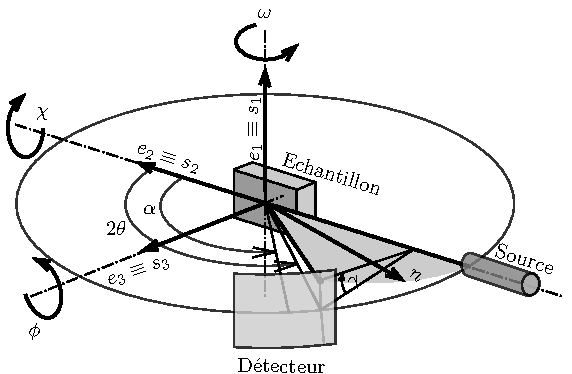
\includegraphics{figures/bases.pdf}
\caption{Schematic diagram showing a sample placed in a diffraction goniometer. When the goniometric angles $\chi$, $\phi$ and $\omega$ are null, the vectors of the base attached to the sample coincide with those of the base attached to the goniometer. }
\label{fig_bases}
\end{figure}


To express the results of the stress analysis, it is necessary to associate a coordinate system with the sample. As shown in Figure \ref{fig_bases}, the base $\mathcal{S}$ of this coordinate system, which is formed by three unit vectors $\boldsymbol s_1$, $\boldsymbol s_2$ and $\boldsymbol s_3$, is such that $\boldsymbol s_3$ corresponds to the direction normal to the external surface of the sample while $\boldsymbol s_1$ and $\boldsymbol s_2$ are contained in the plane. The orientation of the measurement direction $\boldsymbol n$ with respect to the sample depends on the goniometric angles that can be controlled by the user. For diffractometers equipped with an Euler cradle, the three goniometric angles are generally denoted $\omega$, $\chi$ and $\phi$. These angles control the rotations of the sample around the axes $\boldsymbol e_1$, $\boldsymbol e_2$ and $\boldsymbol e_3$. For stress analysis, it is necessary to express the components of the measurement direction $\boldsymbol n$ in the base attached to the sample. This is commonly done from the angles $\Phi$ and $\Psi$, which are obtained from the relation (see Figure \ref{fig_echantillon}): 
\begin{equation}
\boldsymbol n =
\begin{bmatrix}
s_\Psi c_\Phi \\
s_\Psi s_\Phi \\
c_\Psi 
\end{bmatrix}_{\mathcal{S}}
=
\begin{bmatrix}
c_\chi c_\phi & c_\omega s_\phi + s_\omega s_\chi c_\phi & s_\omega s_\phi - c_\omega s_\chi c_\phi \\
-c_\chi s_\phi  & c_\omega c_\phi - s_\omega s_\chi s_\phi &   s_\omega c_\phi + c_\omega s_\chi s_\phi\\
s_\chi & -s_\omega  c_\chi & c_\omega  c_\chi  
\end{bmatrix}
\begin{bmatrix}
c_\theta s_\gamma \\
-s_\theta  \\
c_\theta c_\gamma
\end{bmatrix}_{\mathcal{E}}
\end{equation}
The above relation is important in the sense that it allows determining the measurement direction for each pixel ($2 \theta$ and $\gamma$) of the detector according to the orientation of the sample represented by the goniometric angles ($ \omega$, $\chi$ and $\phi$).

\begin{figure}
\centering
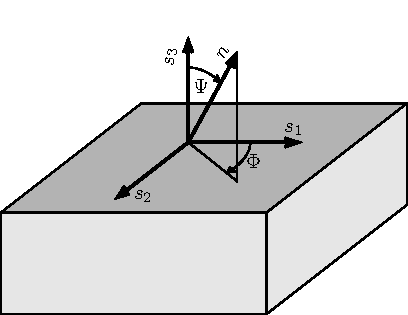
\includegraphics{figures/echantillon.pdf}
\caption{Schematic diagram showing the measurement direction $\boldsymbol n$ in the base associated with a sample. The measurement direction is oriented from the angles $\Psi$ and $\Phi$.}
\label{fig_echantillon}
\end{figure}

\section{Data importation and data integration}

When point or linear detectors are used, stress analysis by diffractometric methods relies on the collection of a set of diffraction profiles. Each diffraction profile, which corresponds to a measurement direction, contains a set of measurement points which give the intensity $I$ of the diffracted beam as a function of twice the Bragg angle $2 \theta$. In the case of area detectors, the input data takes the form of one or more images. Each image consists of a set of pixels whose gray level represents the intensity of the diffracted beam. To exploit the data obtained with an area detector, it is therefore necessary (i) to associate the angles $2 \theta_{i,j}$ and $\gamma_{i,j} $ corresponding to each pixel $(i,j)$ and (ii) to integrate the data to obtain diffraction profiles.

The determination of the angles $2 \theta_{i,j}$ and $\gamma_{i,j}$ for a pixel exploits the results of the calibration of the detector. The calibration provides (i) the distance $r$ between the detector and the goniometric center, (ii) the coordinates $(x_c, y_c) $ of the center of the detector as well as (iii) the dimensions $\Delta_x$ and $\Delta_y$ of pixels. From the calibration data, it is possible to deduce the coordinates $(x_i,y_j)$ of a pixel $(i,j)$ on a two-dimensional detector from the relations:
\begin{align}
&x_{i}= i \times \Delta_x - x_c\\
&y_{j}= j \times \Delta_y-y_c
\end{align}
Also, the distance $r$ from the detector to the goniometric center and the angle $\alpha$, which gives the position of the detector on the goniometric circle, make it possible to determine the angles $2 \theta_{i,j}$ and $\gamma_ {i,j}$ associated with each pixel:
\begin{align}
&2 \theta_{i,j}  = \arccos \left( \frac{x_i \sin \alpha + r \cos \alpha}{r^2+x_i^2+y_j^2} \right) \\
&\gamma_{i,j}  = \text{sign} \left( y_{j}  \right)\arccos \left(  \frac{r \sin \alpha-x_{i} \cos \alpha }{\sqrt{y_{j}^2+(r \sin \alpha-x_{i} \cos \alpha)^2 }} \right)
\end{align}

Data integration requires the construction of diffraction profiles, \textit{i.e.} determining the evolution of the intensity as a function of the angle $2\theta$ for a fixed angle $\gamma$. In practice, it is necessary to introduce tolerances $\Delta 2 \theta$ and $\Delta \gamma$ to decide whether the result of a pixel must be included or not in a diffraction profile. A simple approach (see Figure \ref{fig_detecteur}) for integration consists in considering that the intensity $I (2 \theta )$ for a fixed value of $\gamma$ is obtained by adding the intensities $I_{ i,j}$ of all the pixels $(i,j)$ that satisfy the conditions:
\begin{align}
&2 \theta- \frac{1}{2} \Delta 2 \theta \leq 2 \theta_{i,j}  < 2 \theta+ \frac{1}{2} \Delta 2 \theta \\
&\gamma- \frac{1}{2} \Delta \gamma \leq \gamma_{i,j}  < \gamma+ \frac{1}{2} \Delta \gamma 
\end{align}
Importing a set of images obtained with an area detector therefore makes it possible, after integration, to find a situation similar to that of point or linear detectors, \textit{i.e.} the experimental data consists of different diffraction profiles $I (2 \theta )$ to each of which is associated a quadruplet of angles $(\gamma,\omega,\chi,\phi)$.

\begin{figure}
\centering
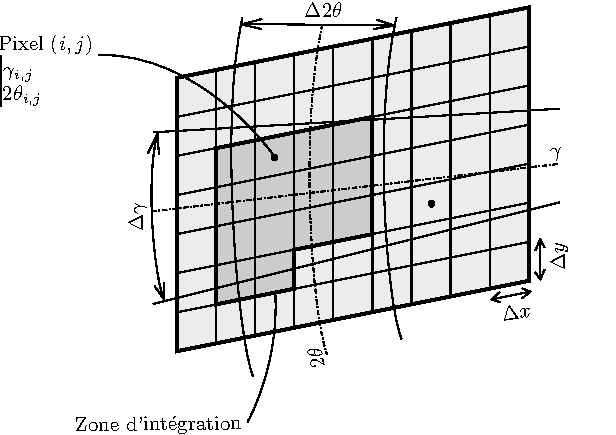
\includegraphics{figures/detecteur.pdf}
\caption{Integration procedure for the construction of a diffraction profile from a two-dimensional image.}
\label{fig_detecteur}
\end{figure}

\section{Correction of diffraction profiles}

Before exploiting diffraction profiles, it is sometimes necessary to apply a set of corrections to the measured intensity. The effect of these corrections is generally grouped in the product $PLA$ which incorporates the polarization, Lorentz and absorption corrections. The polarization correction $P$ depends on the angles $2 \theta$ and $\gamma$ through the relation:
\begin{equation}
P = \frac{\left( 1+\cos^2  2 \theta  \cos^2  2 \theta_m  \right) \cos^2 \gamma +\left( \cos^2  2 \theta  + \cos^2  2 \theta_m  \right) \sin^2 \gamma }{1+\cos^2  2 \theta_m }
\end{equation}
where $\theta_m$ is the Bragg angle associated with the monochromator (the angle $\theta_m$ is zero in the absence of a monochromator).

For conventional diffractometers, the Lorentz factor $L$ is expressed from the angle of incidence $\theta$ as follows:
\begin{equation}
L = \frac{1}{ \sin^2  \theta  }
\end{equation}

Finally, for a sample whose thickness is very large compared to the penetration depth of the radiation, the factor $A$, which accounts for the effect of absorption phenomena, is given by:
\begin{equation}
A = \frac{\cos \beta }{  \left(\cos \beta + \cos \zeta \right)} %\cos \zeta
\end{equation}
with:
\begin{align}
&\cos \beta = \sin \omega \cos \chi\\
&\cos \zeta = \sin 2 \theta \sin \gamma \sin \chi + \sin 2 \theta \cos \gamma \cos \omega \cos \chi -\cos 2 \theta \sin \omega \cos \chi
\end{align}
In the above relation, the angles $\beta$ and $\zeta$ correspond to the angles separating the normal to the sample $\boldsymbol s_3$ respectively from the incident beam and from the diffracted beam. These angles are used to calculate the penetration depth $\tau$ from the relationship:
\begin{equation}
\tau = \frac{\cos \beta \cos \alpha}{ \mu \left(\cos \beta + \cos \zeta \right)} %\cos \zeta
\end{equation}
where $\mu$ is the linear absorption coefficient.

The corrected intensity $i$ is then deduced from the measured intensity $I$ from the relationship:
\begin{equation}
i = \frac{I}{PLA \times t}
\end{equation}
where $t$ represents the counting time. Normalization by the counting time provides an intensity whose unit corresponds to a number of counts per unit of time. Although it is not absolutely necessary for the exploitation of diffraction signals, such normalization allows direct comparison between diffraction profiles obtained for different counting times. Also, for the evaluation of statistical uncertainties, it is necessary to know the uncertainty $\delta i$ associated with the intensity measurement $i$. Assuming that the counting of photons is a Poisson process, the uncertainty $\delta i$ is given by:
\begin{equation}
\delta i = \sqrt{\frac{i}{ PLA \times t}}
\end{equation}

In a similar fashion, to overcome the dependence on the wavelength, it is convenient to represent the intensity as a function of the norm $q$ of the diffraction vector which is expressed as a function of the Bragg angle $\theta$ from:
\begin{equation}
q = \frac{4 \pi \sin \theta}{\lambda}
\end{equation}
where $\lambda$ is the wavelength of the radiation used\footnote{When the radiation used contains the contributions of the $K_{\alpha 1}$ and $K_{\alpha 2}$ lines (of respective wavelength $\lambda_{\alpha 1}$ and $\lambda_{\alpha 2}$), the wavelength $\lambda$ is given by the relation $\lambda = (\lambda_{\alpha 1} + r \lambda_{\alpha 2})/(1+r)$, where $r$ is the intensity ratio between these two contributions.}.

The correction step thus makes it possible to obtain a set of diffraction profiles which can then be analyzed to estimate the positions of the diffraction peaks.

\section{Localisation des pics de diffraction}

To assess the stress state, it is necessary to estimate the positions of the diffraction peaks that contribute to a diffraction profile. One possible method consists in adjusting a function $i(q )$ to best represent a diffraction profile. To do this, it is necessary to identify a set of parameters from the experimental data. In general, the parameters can be classified into two categories. Specifically, some parameters are used to describe the $p$ diffraction peaks that make up a profile while others are used to represent the background. It is therefore possible to decompose the function $i$ additively as follows:
\begin{equation}
 i \left(q \right) = b \left(q  \right) + \sum_{hkl} f_{hkl} \left(q  \right)
\end{equation}
where $b$ represents the contribution of the background while $f_{hkl}$ represents the contribution of the $\{ hkl \}$ reflection to the diffracted signal.

For stress analysis, background is usually modeled by a polynomial function of order $n$ that involves $n+1$ parameters:
\begin{equation}
 b \left(q \right) = b_0 + b_1 q + b_2 q^2 + ...+ b_n q^n
\end{equation}
where the $b_i$ (with $i=0, ... n$) are the background parameters. Also, to represent the diffraction peaks, different functions $f_{hkl}$ are commonly used (see Table \ref{tab_fonction}). Though the number of parameters $m$ used by these functions may vary, they always use at least an intensity parameter $i_{hkl}$, a position parameter $q_{hkl}$ and a width parameter $w_{hkl}$. Additional parameters can be included to control the shape and asymmetry of diffraction peaks. Also, to precisely localize a diffraction peak, it is sometimes necessary to take into account the doublet $K_{\alpha 1} / K_{\alpha 2}$. To do this, the function $f_{hkl} $ associated with the reflection $\{ hkl \}$ is broken down into two contributions:
\begin{equation}
f_{hkl} \left(q \right) = f^1_{hkl} \left(q \right) + r f^2_{hkl} \left(q \right)
\end{equation}
% \begin{equation}
% f_{hkl} \left(q , a_0, a_1, a_2...\right) = f^1 \left(q , a_0, a_1, a_2...\right) + r f^2_{hkl} \left(q, a_0, a_1 \times \lambda_{\alpha 2} / \lambda_{\alpha 1}, a_2... \right)
% \end{equation}
where $r$ denotes the intensity ratio between the contributions $K_{\alpha 1}$ and $K_{\alpha 2}$. The functions $f^1_{hkl}$ and $f^2_{hkl}$ are identical in the sense that they use the same parameters. However, the position of the contribution $K_{\alpha 2}$ is shifted with respect to that of $K_{\alpha 1}$\footnote{If the position of the contribution $f^1_{hkl}$ is $a_1^{hkl}$, that of the contribution $f^2_{hkl}$ corresponds to $ a_1^{hkl}\times \lambda_{\alpha 2} / \lambda_{\alpha 1}$.}. The magnitude of this shift depends on the ratio between the wavelengths $\lambda_{\alpha 1}$ and $\lambda_{\alpha 2}$.

\begin{table}
\centering
\begin{tabular}{ll}
\hline
Function & Definition \\
\hline
& \\
Gauss & \\
\quad Symmetric & $g_s (x)=i \exp \left( - \ln 2 \left( \frac{x-q}{w}\right)^2\right)$ \\
& \\
\quad Asymmetric & $g_a(x)=i \exp \left( - \ln 2 \left( \frac{x-q}{w}\right)^2\right)$ si $x \geq q$ \\
& $g_a(x)=i \exp \left( - \ln 2 \left( \frac{x-q}{w'}\right)^2\right)$ si $x < q$ \\
& \\
\hline
& \\
Lorentz & \\
\quad Symmetric & $l_s(x)= i \left(   1+ \left(\frac{x-q}{w}\right)^2\right)^{-1}$ \\
& \\
\quad Asymmetric & $l_a(x)= i \left(   1+ \left(\frac{x-q}{w}\right)^2\right)^{-1}$ si $x \geq q$ \\
& $l_a(x)= i \left(  1+ \left(\frac{x-q}{w'}\right)^2\right)^{-1}$ si $x < q$ \\
& \\
\hline
& \\
Pseudo-Voigt & \\
\quad Symmetric & $v_s(x)=(1 -s) g_s+ s l_s$ \\
& \\
\quad Asymmetric & $v_a(x)=(1 -s) g_a+ s l_a$  \\
& \\
\hline
& \\
Pearson VII & \\
\quad Symmetric & $p_s(x)=i \left(   1+ \left(\frac{x-q}{w}\right)^2 \left( 2^{1/s}-1\right)\right)^{-s}$  \\
& \\
\quad Asymmetric & $p_a (x) =i \left(   1+ \left(\frac{x-q}{w}\right)^2 \left( 2^{1/s}-1\right)\right)^{-s}$ si $x \geq q$  \\
 & $p_a(x)=i \left(   1+ \left(\frac{x-q}{w'}\right)^2 \left( 2^{1/s}-1\right)\right)^{-s}$ si $x <q$  \\
 & \\
\hline
\end{tabular}
\caption{List of functions commonly used to describe a diffraction peak. The variable on which the function depends is noted $x$. The parameters $i$, $q$, $w$, $w'$ and $s$ respectively control the intensity, the position, the half-widths (right and left) and the shape of a diffraction peak.}
\label{tab_fonction}
\end{table}

The localization step must \textit{in fine} lead to a set of parameters that best describe a diffraction profile. The total number of parameters corresponds to the sum of the number of parameters necessary for the background (\textit{i.e.} $n+1$) and the number of parameters necessary for the description of all the diffraction peaks (\textit{i.e.} $m \times p$). These parameters are obtained by an optimization procedure which seeks to minimize the quadratic difference between the experimental intensity values and those calculated from the chosen modeling function. Besides the optimal values of the parameters, the optimization procedure also provides the associated statistical uncertainties.

\section{Stress evaluation}

The evaluation of stresses within a polycrystalline material is based on the calculation of the elastic strains resulting from the application of a state of stress. The lattice strain $\varepsilon_{hkl}$ of a family of equivalent lattice planes $\{hkl\}$ along the measurement direction $\boldsymbol n$ is calculated from the lattice spacing $d_{hkl} $ using the relation:
\begin{equation}
\varepsilon_{hkl} (\boldsymbol n) = \frac{d_{hkl}(\boldsymbol n)}{d^0_{hkl}}-1
\end{equation}
where $d^0_{hkl}$ represents the lattice spacing in the stress-free state. The localization step described above does not directly provide the lattice spacings $d_{hkl}$ but the positions $q_{hkl}$ (as well as the associated uncertainties) of the peaks which make up the diffraction profiles of an analysis. These two quantities are linked to each other by:
\begin{equation}
q_{hkl} (\boldsymbol n) = \frac{2 \pi}{d_{hkl}(\boldsymbol n)}
\end{equation}
The previous relation allows expressing lattice strains as follows:
\begin{equation}
\varepsilon_{hkl} (\boldsymbol n) = \frac{q^0_{hkl}}{q_{hkl}(\boldsymbol n)}-1
\label{eq_strain_q}
\end{equation}
where $q^0_{hkl}$ represents the position of the diffraction peak $\{hkl\}$ in the the stress-free state.

Lattice strains can be expressed as a function of the stress tensor $\boldsymbol \sigma$ from the tensor $\boldsymbol F_{hkl}$. The latter tensor, which characterizes the stiffness of a material along a unit direction $\boldsymbol n$ for a particular set of lattice planes $\{hkl\}$, is given by:
\begin{equation}
\varepsilon_{hkl} (\boldsymbol n) = \boldsymbol F_{hkl} (\boldsymbol n) : \boldsymbol \sigma
\label{eq_strain_stress}
\end{equation}
The tensor $\boldsymbol F_{hkl}$ is expressed from the Young's modulus $E_{hkl}$ and the Poisson's ratio $\nu_{hkl}$ using the relation\footnote{The tensor $\boldsymbol F_{hkl}$ can also be determined from the crystallographic elasticity constants using the relations $1/2 s_{2,hkl}= (1+\nu_{hkl})/E_{hkl}$ and $ s_{1,hkl} = -\nu_{hkl}/E_{hkl}$.}:
\begin{equation}
\boldsymbol F_{hkl} (\boldsymbol n) = \frac{1+\nu_{hkl}}{E_{hkl}} \boldsymbol n \otimes \boldsymbol n - \frac{\nu_{hkl}}{E_{hkl}} \boldsymbol I 
\end{equation}

The linear system that allow determining the stress state $\boldsymbol \sigma$ is obtained by combining relations \eqref{eq_strain_q} and \eqref{eq_strain_stress}, which leads to:
\begin{equation}
q^0_{hkl}-q_{hkl}(\boldsymbol n) =q_{hkl}(\boldsymbol n) \boldsymbol F_{hkl} (\boldsymbol n) : \boldsymbol \sigma
\end{equation}
Different assumptions can be adopted for the resolution of this linear system. First, it is possible to assume that the stress tensor takes a specific form, in particular that some components are zero. The commonly used stress states are specified in Table \ref{tab_contrainte}.

\begin{table}
\centering
\begin{tabular}{lll}
\hline
\hline
\\[-1em]
Stress state & Surface & Non-zero components\\
\hline
\\[-1em]
Uniaxial along $\boldsymbol s_1$ & Free & $\sigma_{11}$ \\
\hline
\\[-1em]
Uniaxial along $\boldsymbol s_2$ & Free & $\sigma_{22}$ \\
\hline
\\[-1em]
Biaxial along $\boldsymbol s_1$ et $\boldsymbol s_2$ & Free & $\sigma_{11}$, $\sigma_{12}$ and $\sigma_{22}$ \\
\hline
\\[-1em]
Triaxial & Free & $\sigma_{11}$, $\sigma_{12}$, $\sigma_{22}$, $\sigma_{23}$ and $\sigma_{31}$\\
\\[-1em]
 & Constrained & $\sigma_{11}$, $\sigma_{12}$, $\sigma_{22}$, $\sigma_{23}$, $\sigma_{33}$ and $\sigma_{31}$\\
\hline
\hline
\end{tabular}
\caption{Specific stress states that can be used for stress analysis. The presence of a free surface assumes that the normal stress $\sigma_{33}$ is zero.}
\label{tab_contrainte}
\end{table}

Also, in many practical situations, the reference positions $q^0_{hkl}$ of the various lattice planes which contribute to the diffraction profiles are not precisely known. These reference positions then constitute unknowns of the stress analysis problem. They must therefore be determined from the positions $q_{hkl}$ in the same way as the stress state. To do this, it is necessary to assume that the external surface of the sample is free and that the corresponding normal stress is zero (\textit{i.e.} $\sigma_{33}=0$). Nevertheless, for the rare cases where the reference positions are known, the reference positions are considered as input data in the same way as the $q_{hkl}$ positions.

Whatever the assumptions used, the determination of the stress state takes the form of a linear problem whose resolution leads to the stress tensor $\boldsymbol \sigma$, as well as to the associated statistical uncertainty $\delta \boldsymbol \sigma$, from the positions $q_{hkl}$ of the diffraction peaks and the associated statistical uncertainties $\delta q_{hkl}$.


\chapter{Graphical user interface}

The X-Light graphical interface is described in this second chapter. The packages needed for installation are first listed. The functions contained in the different tabs that appear in the interface are then detailed. The format of the files that make up the X-Light database is explained in the last part of this chapter.


\section{Installation and execution}

The X-light software is written in Python language. To work properly, X-light requires Python version 3.7 (or higher). Also, prior installation of the following packages is required~:
\begin{itemize}
\item{numpy (1.19 or higher),}
\item{matplotlib (3.5 or higher),}
\item{PySide6 (6.1 or higher),}
\item{scipy (1.6 or higher),}
\item{numba (0.54 or higher).}
\end{itemize}
The graphical interface is launched from the \texttt{X-light} directory using the command~:\\ 
\texttt{Python -m xlight}

\section{Utilization}

The graphical interface of X-Light (see Figure \ref{fig_import}) takes the form of four tabs (\texttt{Import}, \texttt{Inspect}, \texttt{Localize} and \texttt{Evaluate}). Each of these tabs is associated with one of the stress analysis steps. Specifically, the first tab allows importing X-ray diffraction data. The second tab provides useful tools for the inspection of the diffraction profiles contained in the data files. The third tab contains all aspects related to the localization of diffraction peaks. The evaluation of the stress state is carried out from the last tab.


\subsection{Importation}

The import tab contains two commands (\texttt{Import data} and \texttt{Clear data}). Data files are read from the \texttt{Import data} command. The file formats accepted by X-Light are \textit{nja}, \textit{uxd} and \textit{gfrm}. It is possible to perform a stress analysis using data from different files. These files can be imported all at once or in several times using the \texttt{Import data} command. When the files correspond to images (\textit{gfrm}), import requires specifying the dimensions $\Delta 2 \theta$ and $\Delta \gamma$ of the integration window. Also, the wavelengths corresponding to the anode used to generate the radiation should be specified. To do this, X-Light uses a database that contains the characteristics of common anodes (see \ref{sec_fichieranode}). For data obtained from a 2D detector, the X-Light database must also include the corresponding detector and the associated calibration data (see \ref{sec_fichierdetecteur}).

The command \texttt{Clear data} erases all data, as well as the associated results. This command is useful to perform multiple stress analyzes without having to restart X-Light.

\begin{figure}[h!]
\centering
\scalebox{0.18}{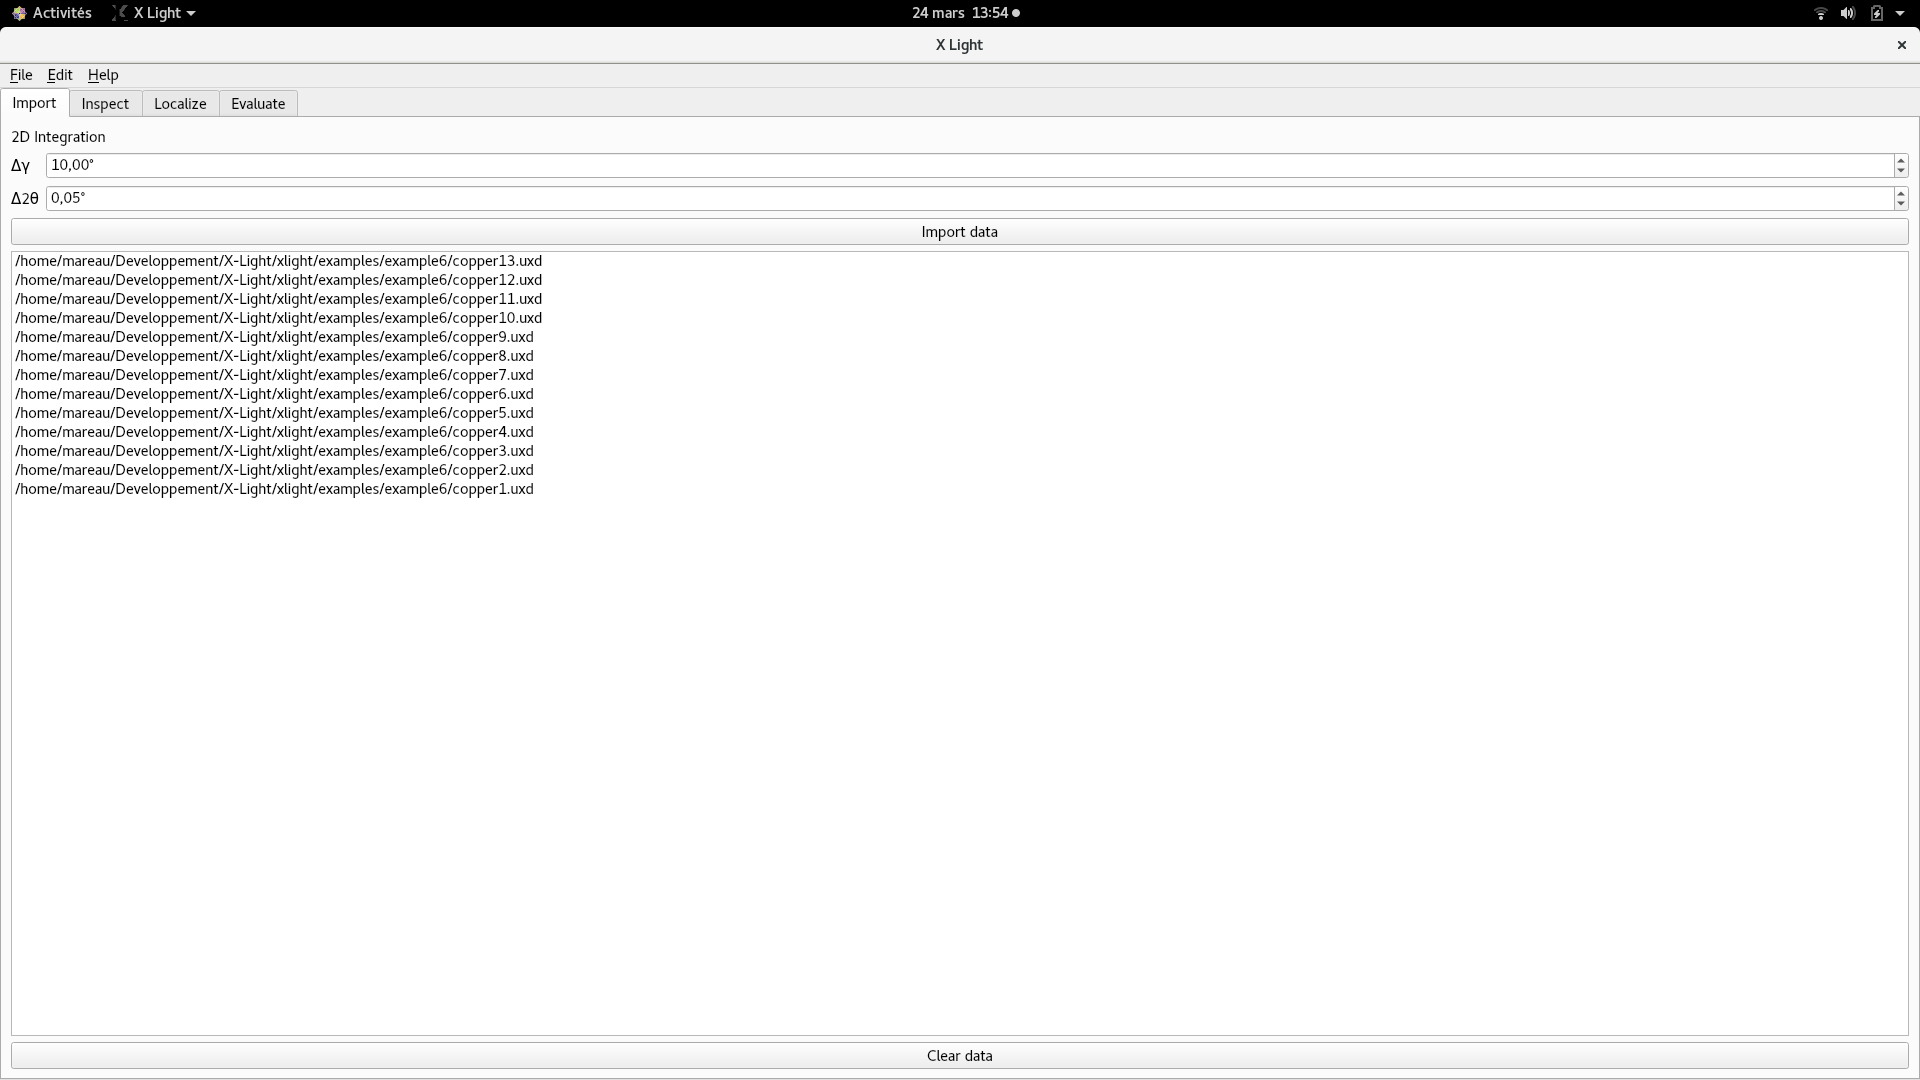
\includegraphics{figures/import.png}}
\caption{View of the import tab of the X-Light interface.}
\label{fig_import}
\end{figure}

\subsection{Inspection}

\label{sec_visualisation}

The diffraction profiles obtained after import are visible in the form of diagrams representing the intensity $I$ as a function of the angle $2\theta$ from the inspection tab (see Figure \ref{fig_inspect}). The data associated with each profile (wavelength, goniometric angles) is presented to the right of the diagram, which also includes zoom and pan functionality. It is possible to switch between the different profiles from the commands placed above the diagram $I-2\theta$. It is important to note that the graphs are supplemented after the localization step by the modeled profiles, which are thus added to the experimental profiles. The \texttt{Enabled/Disabled} option enables/disables a diffraction profile. Data obtained from disabled profiles is not considered for stress evaluation.

\begin{figure}[h!]
\centering
\scalebox{0.18}{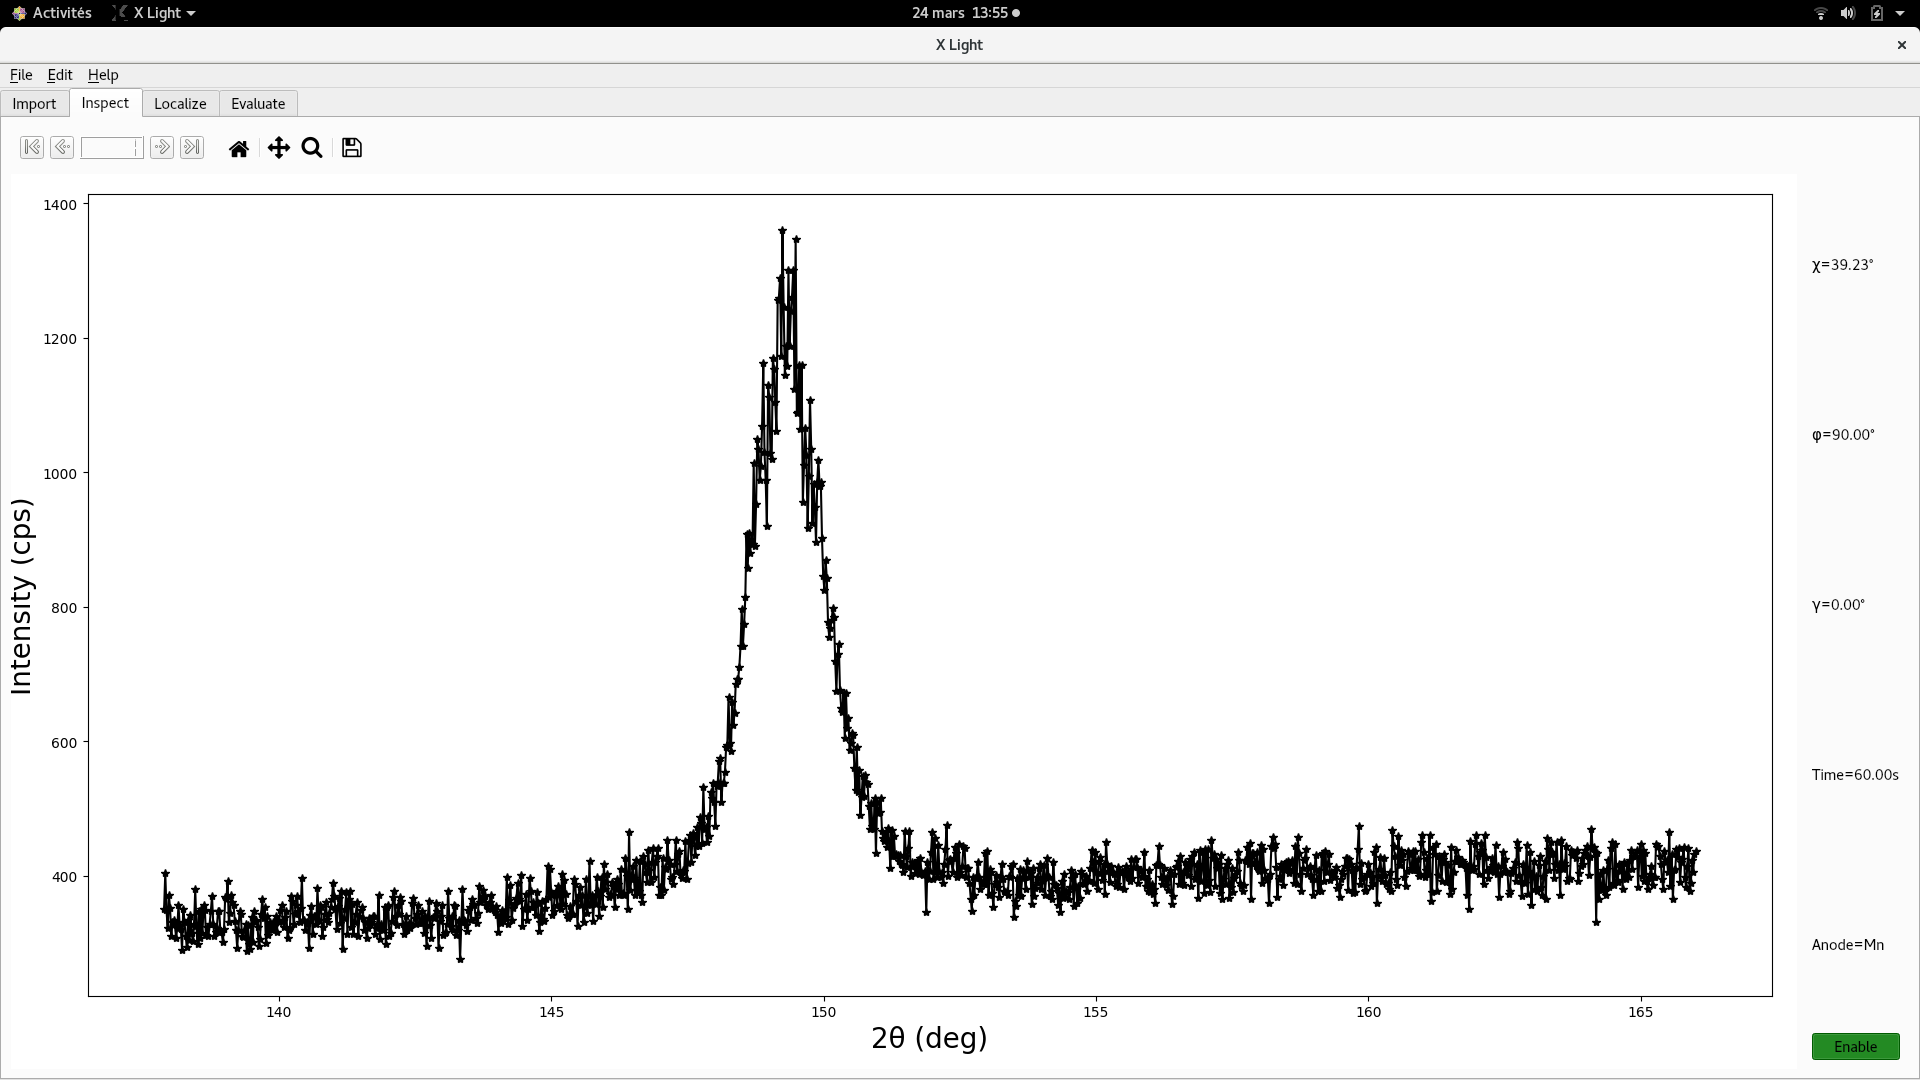
\includegraphics{figures/inspect.png}}
\caption{View of the inspection tab of the X-Light interface.}
\label{fig_inspect}
\end{figure}

\subsection{Localization}

The options available for determining diffraction peak positions are contained in the tab of the same name (see Figure \ref{fig_localize}). The user can choose to apply some corrections (\texttt{Lorentz}, \texttt{Polarization}, \texttt{Absorption}) to the diffraction profiles before the localization step. By default, no correction is applied to diffraction profiles.

For the localization of diffraction peaks, X-light uses the material files available in the database (see \ref{sec_fichiermateriau}). Specifically, from the lattice parameters of the selected metallurgical phase (material), X-Light determines the theoretical positions of the different families of $\{hkl\}$ lattice planes. For each profile, X-Light is then able to identify the planes that should contribute to the diffracted signal. 

\begin{figure}[bh!]
\centering
\scalebox{0.18}{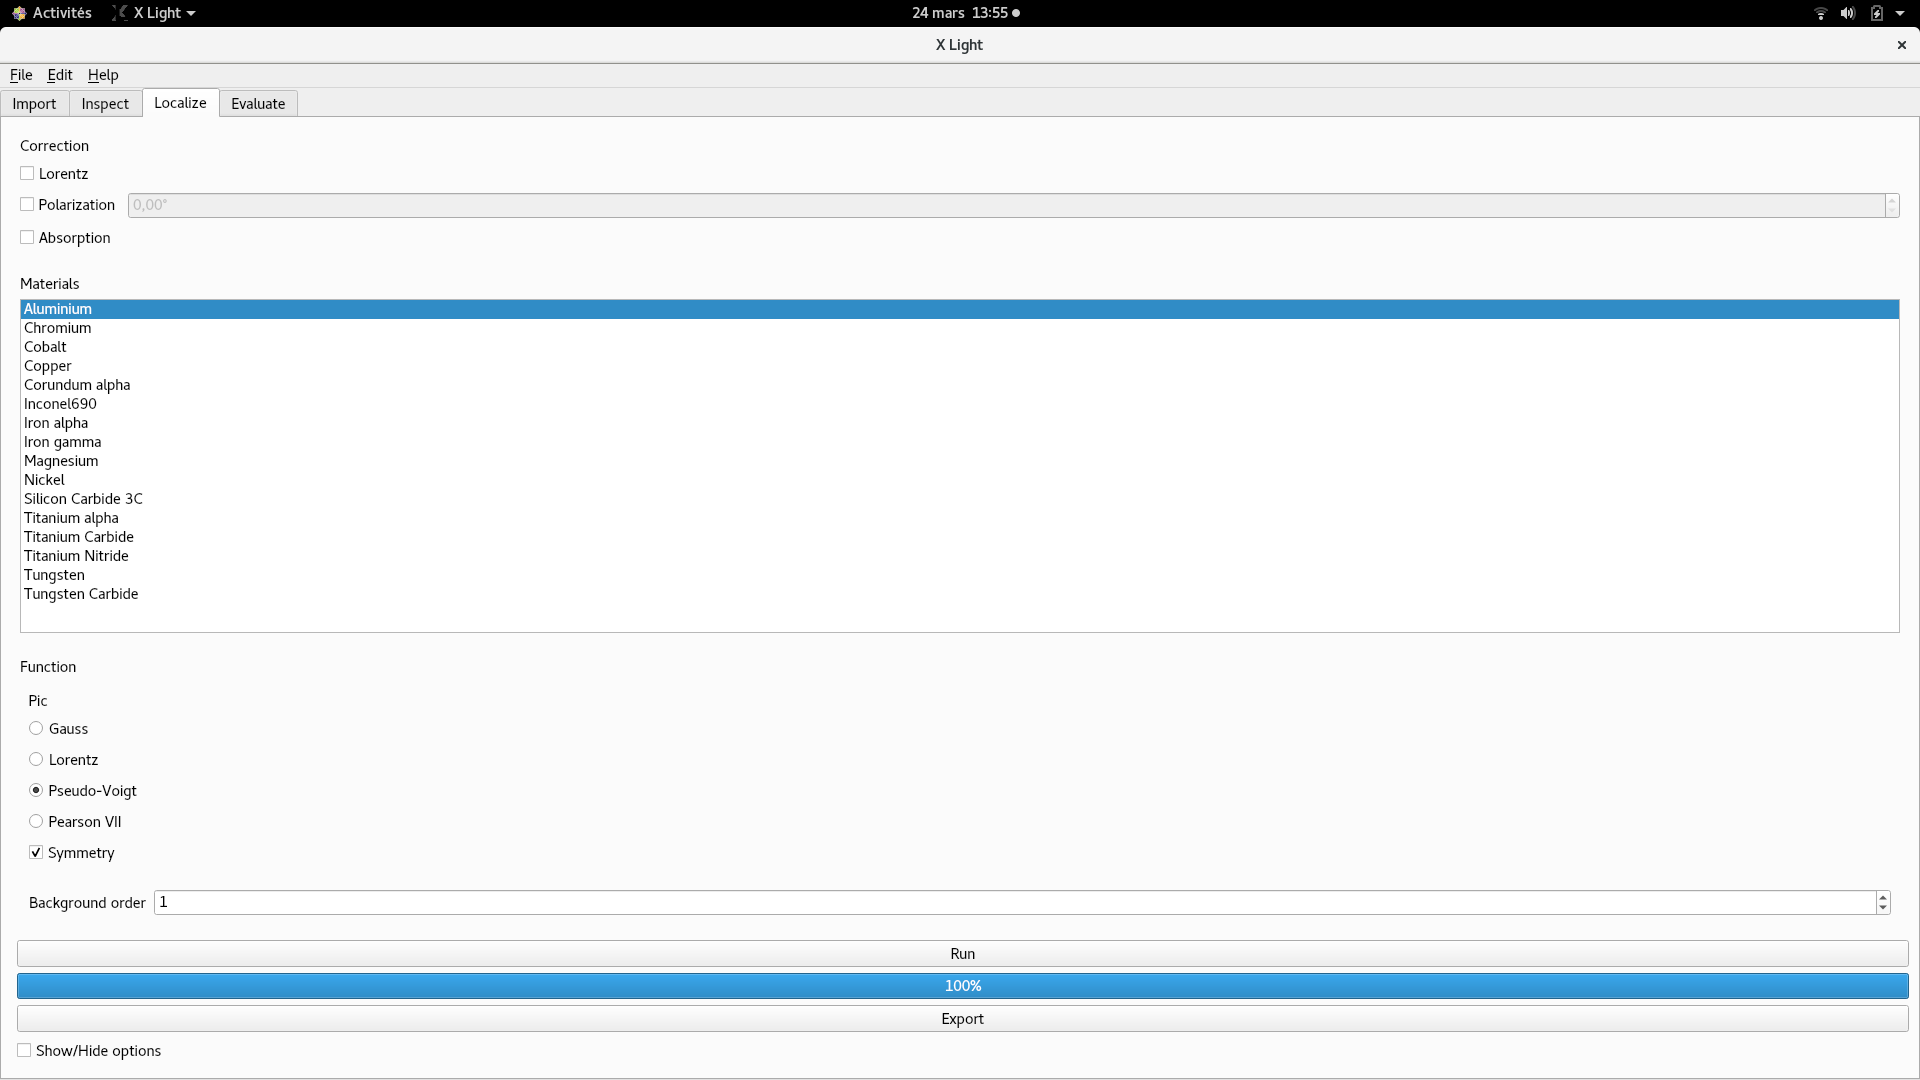
\includegraphics{figures/localize.png}}
\caption{View of the localization tab of the X-Light interface.}
\label{fig_localize}
\end{figure}

The precise localization of diffraction peaks requires indicating the peak modeling function (\texttt{Gauss}, \texttt{Lorentz}, \texttt{Pseudo-Voigt} or \texttt{Pearson VII}) as well as the order of the polynomial function used (\texttt{Background order}) to represent the background. An additional option can be activated to indicate whether the diffraction peak modeling function is symmetric or not. It should be noted that only one type of function can be used for all the data in an analysis.

The application of the corrections then the localization are carried out by X-Light only when the command \texttt{Run} is launched. X-Light uses a global localization procedure in the sense that the parameters of background and diffraction peaks are adjusted simultaneously. After the localization step, it is possible to compare the experimental data to the modeling in the visualization tab (see \ref{sec_visualisation}). Localization results can also be exported to a text file using the \texttt{Export} command.

X-light uses an optimization procedure to determine the parameters (peak and background description) of a diffraction profile. This optimization procedure requires initial estimates of these parameters. The initial estimate of the background parameters is based on an iterative procedure, which uses a tolerance defining the points to be considered to obtain this estimate. The value of this tolerance is controlled from the advanced options (\texttt{Show/Hide options} then \texttt{Background tolerance}). X-light obtains a first estimate of the background parameters from all the data contained within a profile. It then excludes all the points whose intensity is, within the relative tolerance, greater than the background. It then performs a second estimate of the background parameters with a reduced number of experimental points. Points whose intensity is superior to the background are again excluded. This iterative procedure is repeated until the number of points used to evaluate the background parameters remains constant. X-Light also uses the data available in the vicinity of the expected position of each peak to estimate the corresponding position, intensity and width in each diffraction profile. This first estimate is obtained from a center of gravity method, applied to the data contained in a window centered on the expected position. The relative size of this window is controlled from the advanced options \texttt{Show/Hide options} then \texttt{Peak tolerance}. Thus, if the tolerance is denoted by $\theta$, X-light uses the data whose position is between $(1-\theta)\times q^0_{hkl}$ and $(1+\theta)\times q^0_{hkl}$ to determine approximately the position, intensity and width of the diffraction peak associated with the $\{hkl\}$ lattice planes.

\subsection{Stress evaluation}

The evaluation of the stress state is possible as soon as the localization of the diffraction peaks has been carried out. The evaluation tab (see Figure \ref{fig_evaluate}) allows the user to make an assumption regarding the stress state. The possible stress states are presented in Table \ref{tab_contrainte}. The \texttt{Run} command is used to calculate the stress state and the associated uncertainties. Besides the matrix representation of the results, the evaluation tab also gives the von Mises and Tresca equivalent stresses as well as the hydrostatic pressure. If another assumption regarding the stress state is adopted, the command \texttt{Run} has to be pressed to update the results.


\begin{figure}[th!]
\centering
\scalebox{0.18}{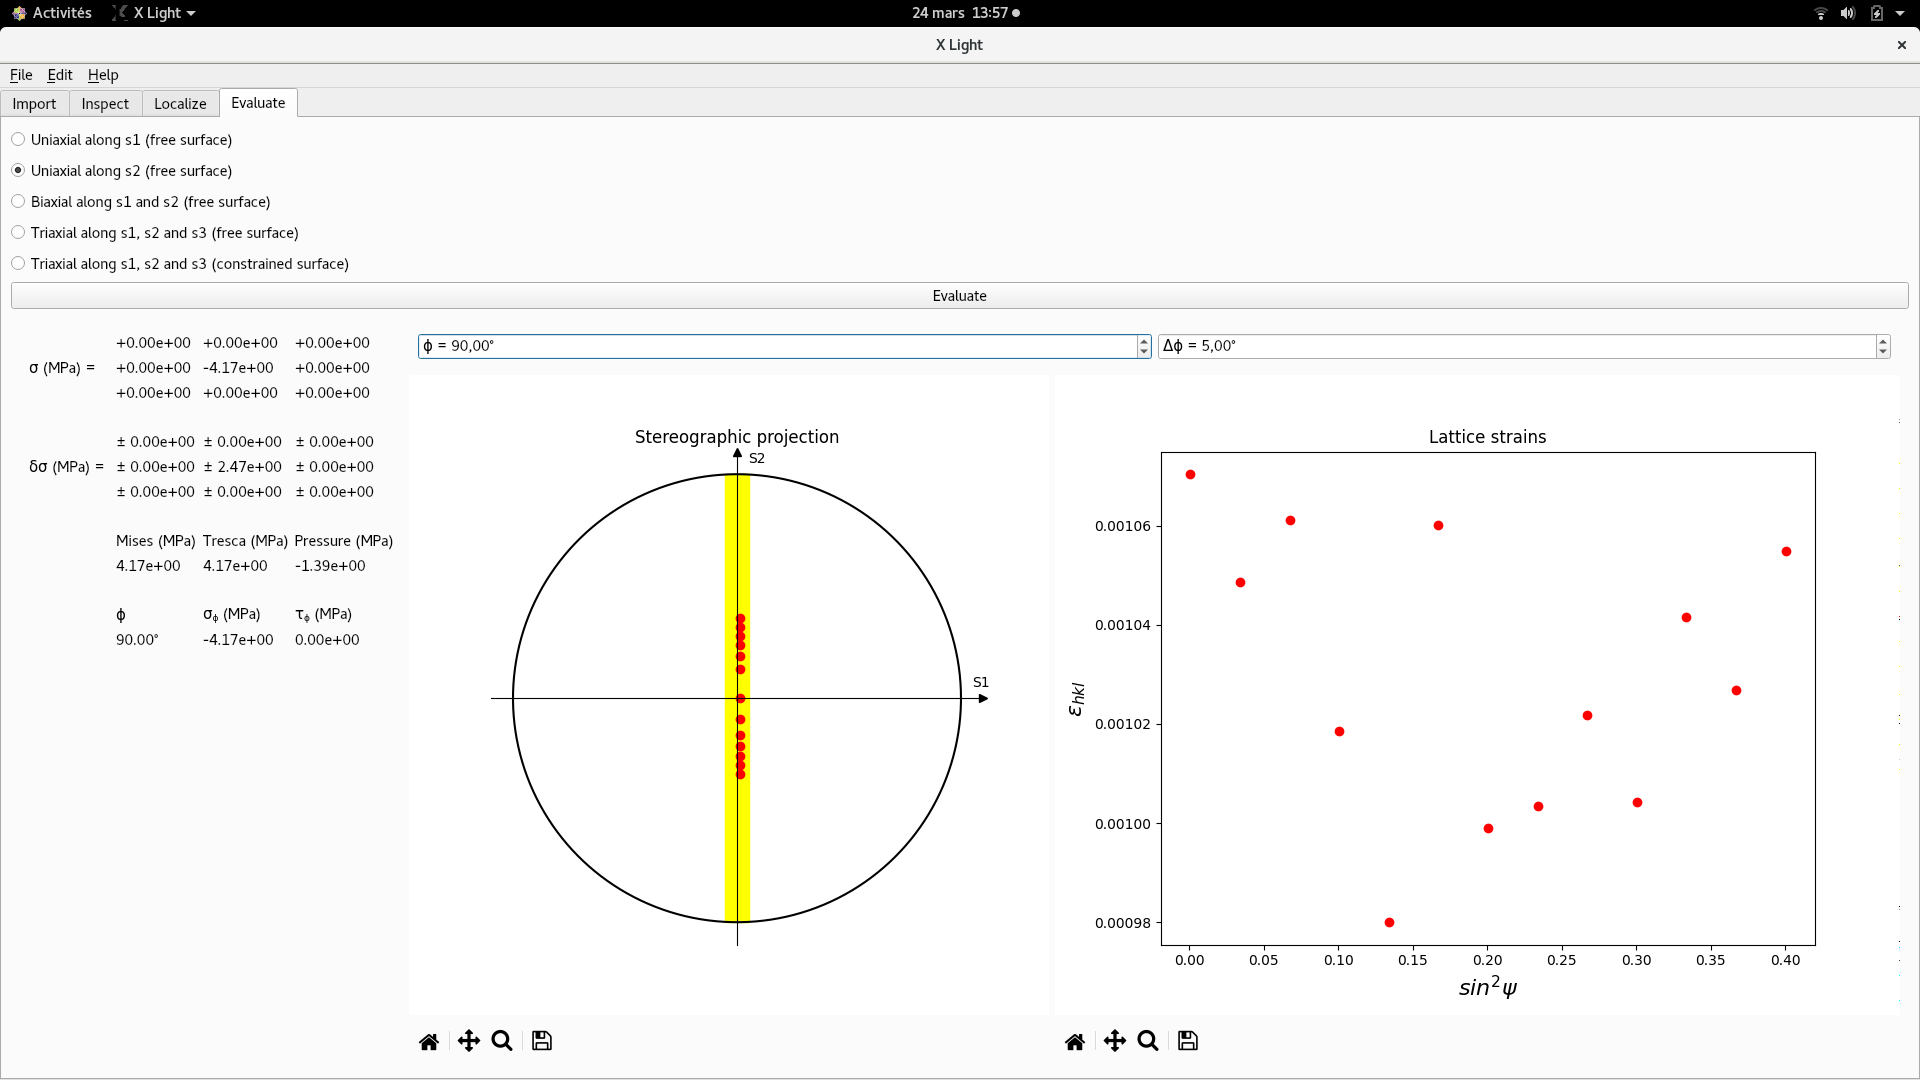
\includegraphics{figures/evaluate.png}}
\caption{View of the evaluation tab of the X-Light interface.}
\label{fig_evaluate}
\end{figure}

The measurement directions corresponding to the different diffraction peaks are displayed on a pole figure, which represents the measurement direction corresponding to each diffraction peak. This representation makes it possible to distinguish between enabled and disabled profiles. Also, the lattice strains $\varepsilon_{hkl}$ obtained for the different diffraction peaks are displayed in a diagram $\varepsilon_{hkl}-\sin^2 \Psi$. On this diagram, the strains associated with an angle $\Phi$, subject to a certain tolerance $\pm \Delta \Phi/2$, are grouped together. Both of these values can be controlled through the interface.

\section{Database}

When performing a stress analysis, X-Light uses a number of files which form the software database. The user can add as many files as needed. However, they must be stored in the appropriate directories. Also, the addition of new files in the database is only effective the next time the software is started.

\subsection{Anode files}

Anode files are contained in the \textit{database/anodes} directory. They contain the values of the wavelengths $K_{\alpha 1}$ and $K_{\alpha 2}$ as well as the intensity ratio $r$ between these wavelengths. The name of the file must be of the type \textit{Xy.txt} where \textit{Xy} designates the chemical symbol of the element used to generate the radiation. For example, the content of the file \textit{Mo.txt} is~:\\
\texttt{***Mo wavelength (Ka1, Ka2, R)} \\
\texttt{0.709300   0.713590  0.5}

\label{sec_fichieranode}

\subsection{Detector files}

Detector files are contained in the \textit{database/detectors} directory. They provide all the information regarding two-dimensional detectors, namely:
\begin{itemize}
\item{the number of pixels in the horizontal and vertical directions,}
\item{the pixel sizes in horizontal and vertical directions,}
\item{the coordinates of the center of the detector,}
\item{the distance between the center of the detector and the goniometric center,}
\item{the parameters of the octahedral mask which allows to define the active zone of the detector.}
\end{itemize}
It is important to know that these parameters correspond to default values. If different values are found when importing data, these new values replace the default values. For example, the description of a VANTEC V500 detector is given by ~:\\
\texttt{***DETECTOR: PXC-V500} \\
\texttt{***NUMBER OF PIXELS (nx, ny)} \\
\texttt{2048     2048} \\
\texttt{***PIXEL SIZE (deltax, deltay)} \\
\texttt{0.068    0.068} \\
\texttt{***DETECTOR CENTER (xc, yc)} \\
\texttt{1008.661      1011.721} \\
\texttt{***DISTANCE TO DETECTOR (d)} \\
\texttt{222.1785} \\
\texttt{***OCTMASK (MinX, MinX+Y, MinY, MaxX-Y, MaxX, MaxX+Y, MaxY, MaxY-X)} \\
\texttt{36  627  14  1416  2007  3458   2028  1415 } \\

\label{sec_fichierdetecteur}

\subsection{Material files}

Materials files are stored in the \textit{database/materials} directory. Each file is associated with a specific material. It contains information related to the nature of the lattice system (\textit{CUBIC}, \textit{HEXAG}, \textit{TRIGO}, \textit{TETRA}, \textit{ORTHO}, \textit{MONOC} and \textit {TRICL}) as well as the associated lattice parameters ($a$, $b$, $c$, $\alpha$, $\beta$ and $\gamma$). Also, the stiffness constants are given for each family of equivalent lattice planes $\{ hkl \}$ through the Young's modulus and the Poisson's ratio. For illustration purpose, the nickel material file is shown below:\\
\texttt{***Nickel XRD input file} \\
\texttt{*CRYSTAL SYSTEM} \\
\texttt{CUBIC} \\
\texttt{*LATTICE PARAMETERS (a,b,c,alpha,beta and gamma)} \\
\texttt{3.5239   3.5239   3.5239   90.   90.   90.} \\
\texttt{*PLANES (hkl)} \\
\texttt{1  1  1     264000   0.26} \\
\texttt{0  0  2     168000   0.35} \\
\texttt{2  2  0     231000   0.29} \\
\texttt{3  1  1     203000   0.32} \\
\texttt{2  2  2     264000   0.26} \\
\texttt{0  0  4     168000   0.35} \\
\texttt{3  3  1     240000   0.28} \\
\texttt{4  2  0     203000   0.32} \\
\label{sec_fichiermateriau}

% 
% eij=(1+v)/E sij - v/E smm 1ij
% 
% e=eij ni nj = (1+v)/E spq  np nq - v/E spq 1pq ni ni 

%     X-Light is a software dedicated to the evaluation of residual stresses using X-ray diffraction. The
% present document gives practical information on the use of X-Light for data acquired with a 2D
% detector. The calibration of the data is performed using pyFAI module, an open-source python
% module available on the web.
% The evaluation of residual stresses using X-ray diffraction data acquired with a 2D detector requires
% the calibration of the frames. This step consists in assigning to each pixel of the frame angular values
% in the (2θ,γ) space, 2θ being the diffraction angle and γ the azimuth angle, corresponding to (ψ,φ)
% values. In the following document, the distinction is made between the calibrant measurement
% (hereafter named calibrant), and the specimen of interest.


% Fin du document
\end{document}
